\section{Graphics}

\subsection{Points}

Distance in 1-D:
$$ d = \Delta x $$

Distance between two points in 2-D: 
$$ d = \sqrt{\Delta x^2 + \Delta y^2} $$

Distance between two points in 3-D:
$$ d = \sqrt{ \sqrt{\Delta x^2 + \Delta y^2}^2 + \Delta z^2 } = \sqrt{\Delta x^2 + \Delta y^2 + \Delta z^2}$$


\subsection{Geometric objects in matrix notation}

$x=1$ defines a plane, as does $x=2y$. $x=1 \land y=2$ defines a line. 
More generally, the dimension of a geometrical object equals 3 minus the number of equations needed to describe the object.
Informally written: $ dim(obj) = 3 - \#(=) $.

In more rigorous terms, the "number of equations needed to describe the object" is called the rank of the matrix. 3 in our case is the dimension of the space. The geometrical object is really the column-space of the matrix. 


\subsubsection{Plane}

Defined by one point $\vec{b}$ and two lines $\vec{p_1}, \vec{p_2}$: 
$$ P = \{ \vec{x} | \thereis a,b:  \vec{x} = \vec{b} + a\vec{p_1} + b\vec{p_2} \} $$

Or defined by one point $\vec{b}$ and one normal $\vec{n}$:
$$ P = \{ \vec{x} | ( \vec{x} - \vec{b} )\cdot \vec{n} = 0 \} $$


\subsubsection{Line}

Defined by two points: 
$$ L = \{ \vec{x} | \thereis \alpha:  \vec{x} = \vec{b} + \alpha \cdot \vec{\Delta}  \}$$

Or transformed in matrix-notation:
$$ 
\vec{x} = 
\begin{bmatrix}
    \vec{b} & \vec{\Delta}
\end{bmatrix}
\cdot
\myarray{ 1 \\ \alpha }
$$

$$
\begin{bmatrix}
    \vec{b} & \vec{\Delta}
\end{bmatrix}^{-1}
\cdot
\vec{x} = 
\myarray{ 1 \\ \alpha }
$$


\subsubsection{Intersection Line/Plane}

Substituting the definition of a line into the definition of a plane we get:

$$ ( \vec{b_l} + \alpha \cdot \vec{\Delta} - \vec{b_p} )\cdot \vec{n} = 0 $$

This reduces to: 

$$ \alpha = \frac{ ( \vec{b_l} - \vec{b_p} ) \cdot \vec{n} }{ \vec{\Delta} \cdot \vec{n} } $$

Alternatively, we can make use of the two-line-definition of the plane and obtain: 

$$ \vec{b}_p + a\vec{p_1} + b\vec{p_2} = \vec{b}_l + \alpha \cdot \vec{\Delta} $$

$$ \vec{b_l} - \vec{b_p} = \myarray{ \vec{p_1} & \vec{p_2} & \vec{\Delta} } \myarray{a \\ b \\ \alpha} $$

\subsection{Projections}

\subsubsection{Finding a perpendicular}

Having a vector $\vec{a}$, how do we find a vector $\vec{a^T}$ that has the following properties:
\begin{itemize}
    \item $ \vec{a} \cdot \vec{a^T} = 0 $
    \item $ | \vec{a} | = | \vec{a^T} | $
\end{itemize}

These two requirements can be re-expressed as 
\begin{itemize}
    \item $ ax + by = 0 $
    \item $ x^2 + y^2 = a^2 + b^2 $
\end{itemize}
This is a nonlinear system, but still solveable. Indeed, we quickly find: 

$$ \vec{a^T} = \myarray{ -y \\ x } $$


How about the two perpendiculars to a 3d-vector? You can just use \myarray{-y & x & 0 } and \myarray{0 & -z & y}. All possible perpendiculars will be linear combinations of these two.


\subsubsection{Projecting one vector onto another}

Imagine we wanted to know $\alpha$ in the following graphic:

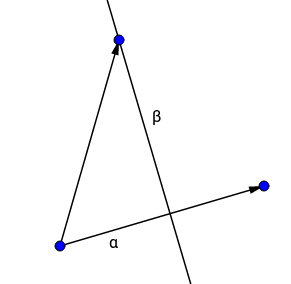
\includegraphics[scale=0.5]{projection.png}

Here, $\alpha$ is the length of vector $\vec{b}$ projected onto $\vec{a}$. How can we find $\alpha$?

The solution lies in imagening the vector $\vec{b}$ being expressed inside a coordinate-system consisting of $\vec{a}$ and $\vec{a^T}$, like so: 

$$ [ \vec{a}, \vec{a^T} ] \myarray{ \alpha \\ \beta } = \vec{b} $$


\subsubsection{Flattening: expressing the points on a 3d-plane in a 2d-system}
From a screen placed in 3d-space we want to obtain a 2d-image that can be displayed on a computer. Consider the plane 
$$ P = {\vec{x} | \vec{x} = \vec{b} + \alpha \vec{p}_1 + \beta \vec{p}_2}$$
A point $\vec{x}_0$ on the screen can be expressed as
$$ \vec{x}_0 = \vec{b} + \alpha \vec{p}_1 + \beta \vec{p}_2 $$
In that case, we just use $\alpha$ and $\beta$ as coordinates. If instead we were using 
$$ P = {\vec{x} | (\vec{x} - \vec{b})\vec{n} = 0} $$
we can still obtain $\vec{p}_1 $ and $ \vec{p}_2$ as 
\begin{align}
    \vec{p}_1 &= \vec{z} \\
    \vec{p}_2 &= \vec{n} \times \vec{z}
\end{align}

\subsection{Rotation}

\subsubsection{In 2d}
To find the rotation matrix $\mtrx{R}_2$  in 2d, you could take the naive approach by taking a generic vector $\begin{bmatrix}x \\ y\end{bmatrix}$ and try to solve this equation: 
\begin{align}
    r = \sqrt{x^2 + y^2} \\
    \theta_0 = \cos^{-1}(x/r) \\
    \mtrx{R}_2 \begin{bmatrix}x \\ y\end{bmatrix} = \begin{bmatrix} 
        r \sin(\theta + \theta_0) \\
        r \cos(\theta + \theta_0)
    \end{bmatrix}
\end{align}
While this is a feasible approach, we can have it much easier. Remember from \ref{changeOfBasis} that 
$$ \vec{v} = \mtrx{T} \vec{v}_T $$
If T is invertible:
$$ \vec{v}_T = \mtrx{T}^{-1} \vec{v} $$
Where:
$$ \mtrx{T}^{-1} = [\vec{x}_T, \vec{y}_T, ...] $$
Specifically, in our case this results in 
$$ \mtrx{R}_2 = \begin{bmatrix} 
    \cos{\theta} & -\sin{\theta} \\
    \sin{\theta} & \cos{\theta}
\end{bmatrix} $$

\subsubsection{In 3d}
While in 2d we only had one axis to rotate around, in 3d we can chose if we want to rotate around x, y, or z. In the general case: 
$$ \mtrx{R}_3 = \mtrx{R}_x \mtrx{R}_y \mtrx{R}_z $$. 
It is easy to obtain $\mtrx{R}_z$, the rotation around the z-axis. Just imagine you viewed everything from above:
$$ \mtrx{R}_x = \begin{bmatrix}
    \cos{\theta} & -\sin{\theta} & 0 \\
    \sin{\theta} & \cos{\theta}   & 0 \\
    0            & 0             & 1
\end{bmatrix}$$
This way we obtain 
$$ 
\left[\begin{matrix}\cos{\left(\beta \right)} \cos{\left(\gamma \right)} & - \sin{\left(\gamma \right)} \cos{\left(\beta \right)} & \sin{\left(\beta \right)}\\\sin{\left(\alpha \right)} \sin{\left(\beta \right)} \cos{\left(\gamma \right)} + \sin{\left(\gamma \right)} \cos{\left(\alpha \right)} & - \sin{\left(\alpha \right)} \sin{\left(\beta \right)} \sin{\left(\gamma \right)} + \cos{\left(\alpha \right)} \cos{\left(\gamma \right)} & - \sin{\left(\alpha \right)} \cos{\left(\beta \right)}\\\sin{\left(\alpha \right)} \sin{\left(\gamma \right)} - \sin{\left(\beta \right)} \cos{\left(\alpha \right)} \cos{\left(\gamma \right)} & \sin{\left(\alpha \right)} \cos{\left(\gamma \right)} + \sin{\left(\beta \right)} \sin{\left(\gamma \right)} \cos{\left(\alpha \right)} & \cos{\left(\alpha \right)} \cos{\left(\beta \right)}\end{matrix}\right]
$$

\subsubsection{Why is there one rotation axis in 2d, but 3 in 3d?}
The rotation axis for any pair of axii that define a plane in space is a third axis perpendicular to that plane. In conventional 2D (XY plane), all rotation is done in the Z axis. 
But what about spherical coordinates? There we need only two angles! ...

\subsection{Implicit versus parameterized representation of bodies}

In geometry, we often represent bodies in set-notation, aka. implicit notation. Consider for example the ellipsoid: 

$$ \left \{\vec{v} | \frac{x^2}{r_1^2} + \frac{z^2}{r_2^2} + \frac{z^2}{r_3^2} = 1 \right \}$$

This body can be parameterized as: 

$$ \begin{bmatrix}
x \\
y \\
z
\end{bmatrix} = 
\begin{bmatrix}
r_1 \cos{\theta} \cos{\phi} \\
r_2 \cos{\theta} \sin{\phi} \\
r_3 \sin{\theta}
\end{bmatrix} $$

In the set notation, the ellipsoid had no parameters (it had $r_1, r_2, r_3$, but these are \emph{constants}). With $\theta$ and $\phi$ we now found two parameters which, when varied over their whole domain $[0\degree, 360\degree]^2$, yield every point in the set. 


Parameterisation means \emph{finding a function of one or more parameters who's range equals the set}. That means nothing other than \emph{putting the vector $\vec{x}$ on the left side}. Conversely, you have an \emph{implicit} equation when you can write the equation such that the left side is $0$ (for clarity: we mean the number $0$, not a zero-vector).


As a sidenote, when you find a set-expression of a body that contains a $thereis$ statement, chances are that this statement already \emph{is} parameterized.


\begin{table}[H]
\centering
\caption{Explicit and parametric set of plane and ellipsoid}
\begin{tabular}{c|cc}
           & implicit                                                 & parametric \\
\hline 
linear     & $\left \{\vec{x} | ( \vec{x} - \vec{b} ) \dot \vec{n} = 0 \right \}$  & $\left \{\vec{x} | \thereis \alpha, \beta: \vec{x} = \begin{bmatrix} \vec{b} && \vec{p}_1 && \vec{p}_2 \end{bmatrix} \begin{bmatrix} 1 \\ \alpha \\ \beta \end{bmatrix}  \right \}$ \\
non-linear & $\left \{\vec{x} | \frac{x^2}{r_x} + \frac{y^2}{r_y} + \frac{z^2}{r_z} = 1 \right \}$ &  $\left \{\vec{x} | \thereis \theta, \phi: \vec{x} = \begin{bmatrix} r_x \cos{\theta} \cos{\phi} \\ r_y \cos{\theta} \sin{\phi} \\ r_z \sin{\theta} \end{bmatrix} \right \}$       
\end{tabular}
\end{table}

We can find more about this topic here: https://en.wikipedia.org/wiki/Implicit\_surface. In this section, we have been careful to never mention the term \emph{explicit}. In this section, we dealt with bodies. But if we only wanted surfaces, that is, bodies where there are never two z values at on x/y spot, there is also the explicit representation $z=f(x,y)$.

\begin{table}[H]
\centering
\caption{Overview of implicit, explicit and parameterized functions}
\begin{tabular}{l|ll|r}
              & in         & out     & notes                                 \\
              \hline
implicit      & x, y, z    &         &                                       \\
explicit      & x, y       & z       & doesn't allow more than one z per x/y \\
parameterized & $\theta, \phi$ & x, y, z &                                      
\end{tabular}
\end{table}

%One neat fact is this: 
%\begin{itemize}
%    \item Take the parameterized version of a body.
%    \item This version can be written as a matrix equation $Ax = b$, by putting all things that can vary %into $x$.
%    \item Calculate the degrees of freedom of this matrix equation: $dof = \#cols - \#rows$.
%    \item The $dof$ equals the minimal amount of parameters that you need to write the parameterized %equation of the body. 
%\end{itemize}
%
%How does one find the minimum amount of parameters for a body, whether it's given implicitly versus explicitly? 
%For an implicit example, consider the case of the ellipsoid again. 
%
%\begin{align*}
%    & \text{ Dimensions:} & 3 \\
% -  & \text{ equations:}  & 1 \\
%\hline  
%   & \text{ Degrees of freedom}   & 2 
% \end{align*}
%
% 
%For an explicit example, consider the line in 3d: $\{\vec{v} | \vec{v} = a \vec{d}\}$
%%
%
%\begin{align*}
%    &  \text{ Dimensions:} & 3  \\
%  - &  \text{ equations:}  & 1  \\
%  - &  \text{ Parameters already in equations:}  & 1 \\
% \hline 
%    &  \text{ Degrees of freedom:}  & 1 
% \end{align*}

